\documentclass[journal,12pt,twocolumn]{IEEEtran}
%
\usepackage{setspace}
\usepackage{gensymb}
\usepackage{xcolor}
\usepackage{caption}
%\usepackage{subcaption}
%\doublespacing
\singlespacing

%\usepackage{graphicx}
%\usepackage{amssymb}
%\usepackage{relsize}
\usepackage[cmex10]{amsmath}
\usepackage{mathtools}
%\usepackage{amsthm}
%\interdisplaylinepenalty=2500
%\savesymbol{iint}
%\usepackage{txfonts}
%\restoresymbol{TXF}{iint}
%\usepackage{wasysym}
\usepackage{hyperref}
\usepackage{amsthm}
\usepackage{mathrsfs}
\usepackage{txfonts}
\usepackage{stfloats}
\usepackage{cite}
\usepackage{cases}
\usepackage{subfig}
%\usepackage{xtab}
\usepackage{longtable}
\usepackage{multirow}
%\usepackage{algorithm}
%\usepackage{algpseudocode}
%\usepackage{enumerate}
\usepackage{enumitem}
\usepackage{mathtools}
%\usepackage{iithtlc}
%\usepackage[framemethod=tikz]{mdframed}
\usepackage{listings}
\let\vec\mathbf


%\usepackage{stmaryrd}


%\usepackage{wasysym}
%\newcounter{MYtempeqncnt}
\DeclareMathOperator*{\Res}{Res}
%\renewcommand{\baselinestretch}{2}
\renewcommand\thesection{\arabic{section}}
\renewcommand\thesubsection{\thesection.\arabic{subsection}}
\renewcommand\thesubsubsection{\thesubsection.\arabic{subsubsection}}

\renewcommand\thesectiondis{\arabic{section}}
\renewcommand\thesubsectiondis{\thesectiondis.\arabic{subsection}}
\renewcommand\thesubsubsectiondis{\thesubsectiondis.\arabic{subsubsection}}

%\renewcommand{\labelenumi}{\textbf{\theenumi}}
%\renewcommand{\theenumi}{P.\arabic{enumi}}

% correct bad hyphenation here
\hyphenation{op-tical net-works semi-conduc-tor}

\lstset{
language=Python,
frame=single, 
breaklines=true,
columns=fullflexible
}



\begin{document}
%

\theoremstyle{definition}
\newtheorem{theorem}{Theorem}[section]
\newtheorem{problem}{Problem}
\newtheorem{proposition}{Proposition}[section]
\newtheorem{lemma}{Lemma}[section]
\newtheorem{corollary}[theorem]{Corollary}
\newtheorem{example}{Example}[section]
\newtheorem{definition}{Definition}[section]
%\newtheorem{algorithm}{Algorithm}[section]
%\newtheorem{cor}{Corollary}
\newcommand{\BEQA}{\begin{eqnarray}}
\newcommand{\EEQA}{\end{eqnarray}}
\newcommand{\define}{\stackrel{\triangle}{=}}
\newcommand{\myvec}[1]{\ensuremath{\begin{pmatrix}#1\end{pmatrix}}}
\newcommand{\mydet}[1]{\ensuremath{\begin{vmatrix}#1\end{vmatrix}}}

\bibliographystyle{IEEEtran}
%\bibliographystyle{ieeetr}

\providecommand{\nCr}[2]{\,^{#1}C_{#2}} % nCr
\providecommand{\nPr}[2]{\,^{#1}P_{#2}} % nPr
\providecommand{\mbf}{\mathbf}
\providecommand{\pr}[1]{\ensuremath{\Pr\left(#1\right)}}
\providecommand{\qfunc}[1]{\ensuremath{Q\left(#1\right)}}
\providecommand{\sbrak}[1]{\ensuremath{{}\left[#1\right]}}
\providecommand{\lsbrak}[1]{\ensuremath{{}\left[#1\right.}}
\providecommand{\rsbrak}[1]{\ensuremath{{}\left.#1\right]}}
\providecommand{\brak}[1]{\ensuremath{\left(#1\right)}}
\providecommand{\lbrak}[1]{\ensuremath{\left(#1\right.}}
\providecommand{\rbrak}[1]{\ensuremath{\left.#1\right)}}
\providecommand{\cbrak}[1]{\ensuremath{\left\{#1\right\}}}
\providecommand{\lcbrak}[1]{\ensuremath{\left\{#1\right.}}
\providecommand{\rcbrak}[1]{\ensuremath{\left.#1\right\}}}
\theoremstyle{remark}
\newtheorem{rem}{Remark}
\newcommand{\sgn}{\mathop{\mathrm{sgn}}}
\newcommand{\rect}{\mathop{\mathrm{rect}}}
\newcommand{\sinc}{\mathop{\mathrm{sinc}}}
\providecommand{\abs}[1]{\left\vert#1\right\vert}
\providecommand{\res}[1]{\Res\displaylimits_{#1}} 
\providecommand{\norm}[1]{\lVert#1\rVert}
\providecommand{\mtx}[1]{\mathbf{#1}}
\providecommand{\mean}[1]{E\left[ #1 \right]}
\providecommand{\fourier}{\overset{\mathcal{F}}{ \rightleftharpoons}}
\providecommand{\ztrans}{\overset{\mathcal{Z}}{ \rightleftharpoons}}

%\providecommand{\hilbert}{\overset{\mathcal{H}}{ \rightleftharpoons}}
\providecommand{\system}[1]{\overset{\mathcal{#1}}{ \longleftrightarrow}}
	%\newcommand{\solution}[2]{\textbf{Solution:}{#1}}
\newcommand{\solution}{\noindent \textbf{Solution: }}
\providecommand{\dec}[2]{\ensuremath{\overset{#1}{\underset{#2}{\gtrless}}}}
\numberwithin{equation}{section}
%\numberwithin{equation}{subsection}
%\numberwithin{problem}{subsection}
%\numberwithin{definition}{subsection}
\makeatletter
\@addtoreset{figure}{problem}
\makeatother

\let\StandardTheFigure\thefigure
%\renewcommand{\thefigure}{\theproblem.\arabic{figure}}
\renewcommand{\thefigure}{\theproblem}


%\numberwithin{figure}{subsection}

\def\putbox#1#2#3{\makebox[0in][l]{\makebox[#1][l]{}\raisebox{\baselineskip}[0in][0in]{\raisebox{#2}[0in][0in]{#3}}}}
     \def\rightbox#1{\makebox[0in][r]{#1}}
     \def\centbox#1{\makebox[0in]{#1}}
     \def\topbox#1{\raisebox{-\baselineskip}[0in][0in]{#1}}
     \def\midbox#1{\raisebox{-0.5\baselineskip}[0in][0in]{#1}}

\vspace{3cm}

\title{ 
%\logo{
%}
Fourier Series
%	\logo{Octave for Math Computing }
}
%\title{
%	\logo{Matrix Analysis through Octave}{\begin{center}\includegraphics[scale=.24]{tlc}\end{center}}{}{HAMDSP}
%}


% paper title
% can use linebreaks \\ within to get better formatting as desired
%\title{Matrix Analysis through Octave}
%
%
% author names and IEEE memberships
% note positions of commas and nonbreaking spaces ( ~ ) LaTeX will not break
% a structure at a ~ so this keeps an author's name from being broken across
% two lines.
% use \thanks{} to gain access to the first footnote area
% a separate \thanks must be used for each paragraph as LaTeX2e's \thanks
% was not built to handle multiple paragraphs
%

\author{Gautam Singh}
% note the % following the last \IEEEmembership and also \thanks - 
% these prevent an unwanted space from occurring between the last author name
% and the end of the author line. i.e., if you had this:
% 
% \author{....lastname \thanks{...} \thanks{...} }
%                     ^------------^------------^----Do not want these spaces!
%
% a space would be appended to the last name and could cause every name on that
% line to be shifted left slightly. This is one of those "LaTeX things". For
% instance, "\textbf{A} \textbf{B}" will typeset as "A B" not "AB". To get
% "AB" then you have to do: "\textbf{A}\textbf{B}"
% \thanks is no different in this regard, so shield the last } of each \thanks
% that ends a line with a % and do not let a space in before the next \thanks.
% Spaces after \IEEEmembership other than the last one are OK (and needed) as
% you are supposed to have spaces between the names. For what it is worth,
% this is a minor point as most people would not even notice if the said evil
% space somehow managed to creep in.



% The paper headers
%\markboth{Journal of \LaTeX\ Class Files,~Vol.~6, No.~1, January~2007}%
%{Shell \MakeLowercase{\textit{et al.}}: Bare Demo of IEEEtran.cls for Journals}
% The only time the second header will appear is for the odd numbered pages
% after the title page when using the twoside option.
% 
% *** Note that you probably will NOT want to include the author's ***
% *** name in the headers of peer review papers.                   ***
% You can use \ifCLASSOPTIONpeerreview for conditional compilation here if
% you desire.




% If you want to put a publisher's ID mark on the page you can do it like
% this:
%\IEEEpubid{0000--0000/00\$00.00~\copyright~2007 IEEE}
% Remember, if you use this you must call \IEEEpubidadjcol in the second
% column for its text to clear the IEEEpubid mark.



% make the title area
\maketitle

%\newpage

\tableofcontents

%\renewcommand{\thefigure}{\thesection.\theenumi}
%\renewcommand{\thetable}{\thesection.\theenumi}

\renewcommand{\thefigure}{\theenumi}
\renewcommand{\thetable}{\theenumi}

%\renewcommand{\theequation}{\thesection}


\bigskip

\begin{abstract}
This manual provides a simple introduction to Fourier Series
\end{abstract}
\section{Periodic Function}
Let 
\begin{align}
	x(t) &= A_0\abs{\sin\brak{2\pi f_0 t}}
	\label{eq:10-orig-diff-def}
\end{align}
\begin{enumerate}[label=\thesection.\arabic*
,ref=\thesection.\theenumi]
\item Plot $x(t)$.

\solution The Python code \texttt{codes/1\_1.py} plots $x(t)$ below.
\begin{figure}[!htp]
    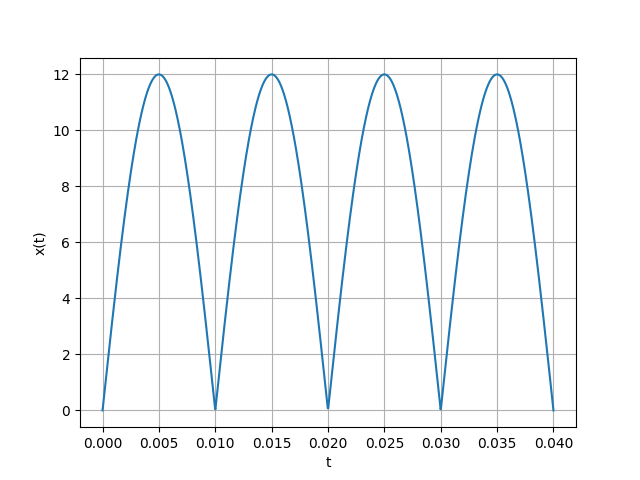
\includegraphics[width=\columnwidth]{figs/1_1.png}
    \caption{$x(t)$}
    \label{fig:xt}
\end{figure}
\item Show that $x(t)$ is periodic and find its period.

\solution From Fig. \eqref{fig:xt}, we see that $x(t)$ is periodic. Further,
\begin{align}
    x\brak{t+\frac{1}{2f_0}} &= A_0\abs{\sin\brak{2\pi f_0\brak{t + \frac{1}{2f_0}}}} \\
                            &= A_0\abs{\sin\brak{2\pi f_0t + \pi}} \\
                            &= A_0\abs{\sin\brak{2\pi f_0t}}
\end{align}
Hence the period of $x(t)$ is $\frac{1}{2f_0}$.
\end{enumerate}
\section{Fourier Series}
Consider $A_0 =12$ and $f_0 = 50$ for all numerical calculations.
\begin{enumerate}[label=\thesection.\arabic*,ref=\thesection.\theenumi]
\item If
\begin{align}
	x(t) = \sum_{k = -\infty}^{\infty}c_ke^{\j2\pi kf_0 t}
\label{eq:one-Z-complex}
\end{align}
show that 
\begin{align}
	c_k = f_0\int_{-\frac{1}{2f_0}}^{\frac{1}{2f_0}}x(t)e^{-\j2\pi kf_0 t}\, dt
\label{eq:one-Z}
\end{align}

\solution We have for some $n \in \mathbb{Z}$,
\begin{align}
    x(t)e^{-\j2\pi nf_0t} = \sum_{k = -\infty}^{\infty}c_ke^{\j2\pi (k - n)f_0 t}
\end{align}
But we know from the periodicity of $e^{\j2\pi kf_0t}$,
\begin{align}
    \int_{-\frac{1}{2f_0}}^{\frac{1}{2f_0}}e^{\j2\pi kf_0 t}\, dt = 
    \frac{1}{f_0}\delta\brak{k} 
\end{align}
Thus,
\begin{align}
    \int_{-\frac{1}{2f_0}}^{\frac{1}{2f_0}}x(t)e^{-\j2\pi nf_0 t}\, dt = 
    \frac{c_n}{f_0} \\
    \implies c_n = f_0\int_{-\frac{1}{2f_0}}^{\frac{1}{2f_0}}x(t)e^{-\j2\pi nf_0 t}\, dt 
\end{align}
\item Find $c_k$ for \eqref{eq:10-orig-diff-def}

\solution Using \eqref{eq:one-Z},
\begin{align}
    c_n &= f_0\int_{-\frac{1}{2f_0}}^{\frac{1}{2f_0}}A_0\abs{\sin\brak{2\pi f_0t}}
    e^{-\j2\pi nf_0t}\, dt \\
        &= f_0\int_{-\frac{1}{2f_0}}^{\frac{1}{2f_0}}A_0\abs{\sin\brak{2\pi f_0t}}
    \cos\brak{2\pi nf_0t}\, dt \nonumber \\
        &+ \j f_0\int_{-\frac{1}{2f_0}}^{\frac{1}{2f_0}}A_0
        \abs{\sin\brak{2\pi f_0t}}\sin\brak{2\pi nf_0t}\, dt \\
        &= 2f_0\int_{0}^{\frac{1}{2f_0}}A_0\sin\brak{2\pi f_0t}\cos\brak{2\pi nf_0t}\, dt \\
        &= f_0A_0\int_{0}^{\frac{1}{2f_0}}\brak{\sin\brak{2\pi\brak{n+1}f_0t}}\, dt \nonumber \\ 
        &- f_0A_0\int_{0}^{\frac{1}{2f_0}}\brak{\sin\brak{2\pi\brak{n-1}f_0t}}\, dt \\ 
        &= A_0\frac{1+\brak{-1}^n}{2\pi}\brak{\frac{1}{n+1} - \frac{1}{n-1}} \\
        &= 
        \begin{cases}
            \frac{2A_0}{\pi\brak{1-n^2}} & n\ \text{even} \\
            0 & n\ \text{odd}
        \end{cases}
        \label{eq:ck-xt}
\end{align}
\item Verify 
	\eqref{eq:one-Z-complex}
	using python.

\solution The Python code \texttt{codes/2\_3.py} verifies \eqref{eq:one-Z-real}.
\begin{figure}[!ht]
    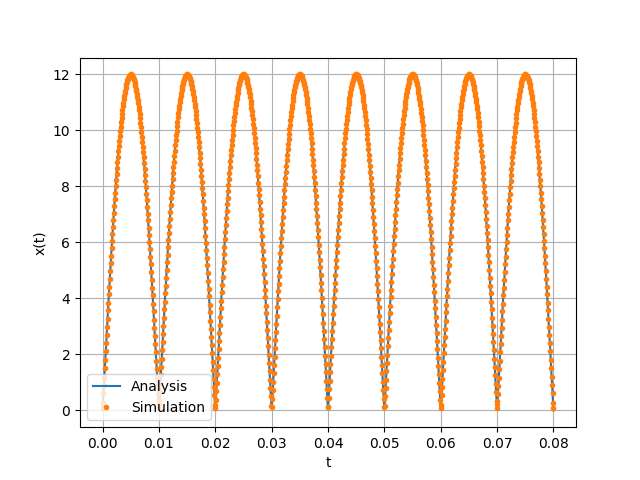
\includegraphics[width=\columnwidth]{figs/2_3.png}
    \caption{Verification of \eqref{eq:one-Z-complex}.}
    \label{fig:ver-complex}
\end{figure}

\item Show that 
\begin{align}
	x(t) = \sum_{k = 0}^{\infty}\brak{a_k\cos{\j2\pi kf_0 t}+b_k\sin{\j2\pi kf_0 t}}
\label{eq:one-Z-real}
\end{align}
and obtain the formulae for $a_k$ and $b_k$.

\solution From \eqref{eq:one-Z-complex},
\begin{align}
    x(t) &= \sum_{k = -\infty}^{\infty}c_ke^{\j2\pi kf_0 t} \\
         &= c_0 + \sum_{k = 1}^{\infty}c_ke^{\j2\pi kf_0t} + c_{-k}e^{-\j2\pi kf_0t} \\
         &= c_0 + \sum_{k = 1}^{\infty}\brak{c_k + c_{-k}}\cos\brak{2\pi kf_0t}  \nonumber \\
         &+ \sum_{k = 0}^{\infty}\brak{c_k - c_{-k}}\sin\brak{2\pi kf_0t}
\end{align}
Hence, for $k \ge 0$,
\begin{align}
    a_k &= 
    \begin{cases}
        c_0 & k = 0 \\
        c_k + c_{-k} & k > 0
    \end{cases} \label{eq:ak} \\
    b_k &= c_k - c_{-k}
    \label{eq:bk}
\end{align}
\item Find $a_k$ and $b_k$ for 
	\eqref{eq:10-orig-diff-def}

\solution From \eqref{eq:one-Z-complex}, we see that since $x(t)$ is even,
\begin{align}
    x(-t) &= \sum_{k = -\infty}^{\infty}c_ke^{-\j2\pi kf_0 t} \\
          &= \sum_{k = -\infty}^{\infty}c_{-k}e^{\j2\pi kf_0t} \label{eq:sub} \\
          &= \sum_{k = -\infty}^{\infty}c_ke^{\j2\pi kf_0 t}
\end{align}
where we substitute $k := -k$ in \eqref{eq:sub}. Hence, we see that 
$c_k = c_{-k}$. So, from \eqref{eq:ak} and \eqref{eq:bk}, for $k \ge 0$,
\begin{align}
    a_k &= 
    \begin{cases}
        \frac{2A_0}{\pi} & k = 0 \\
        \frac{4A_0}{\pi\brak{1 - k^2}} & k > 0,\ k\ \text{even} \\
        0 & \text{otherwise}
    \end{cases} \label{eq:ak-xt}\\
    b_k &= 0
    \label{eq:bk-xt}
\end{align}
\item Verify 
\eqref{eq:one-Z-real}
using python.

\solution The Python code \texttt{codes/2\_6.py} verifies \eqref{eq:one-Z-real}.
\begin{figure}[!ht]
    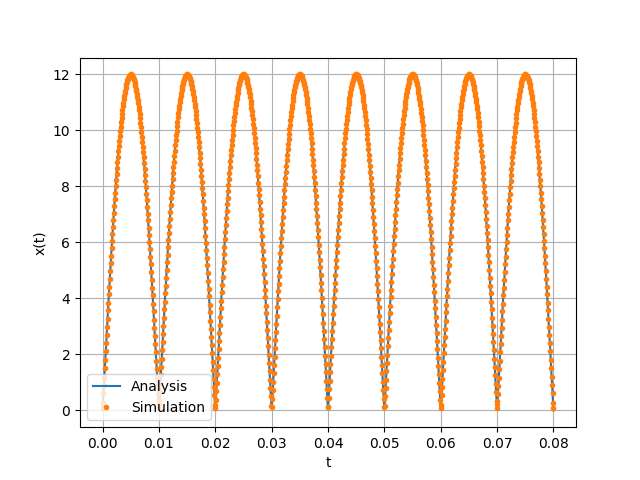
\includegraphics[width=\columnwidth]{figs/2_6.png}
    \caption{Verification of \eqref{eq:one-Z-real}.}
    \label{fig:ver-real}
\end{figure}
\end{enumerate}
\section{Fourier Transform}

\begin{enumerate}[label=\thesection.\arabic*
,ref=\thesection.\theenumi]
\item 
\begin{align}
	\delta(t)&=0, \quad t\neq 0 \\
	\int_{-\infty}^{\infty}\delta(t) \, dt&= 1
\end{align}
\item The Fourier Transform of $g(t)$ is
\begin{align}
G(f)=\int_{-\infty}^{\infty}g(t)e^{-j2\pi ft}\,dt
\label{eq:fourier}
\end{align}
\item Show that 
\begin{align}
    g(t-t_0)&\system{F}G(f)e^{-j2\pi ft_0}
    \label{eq:t-shift}
\end{align}

\solution We write, substituting $u := t-t_0$,
\begin{align}
    g(t-t_0)&\system{F}\int_{-\infty}^{\infty}
            g(t-t_0)e^{-\j2\pi ft}\,dt \\
            &=\int_{-\infty}^{\infty}
            g(u)e^{-\j2\pi f(u + t_0)}\,du \\
            &=G(f)e^{-j2\pi ft_0}
\end{align}
where the last equality follows from \eqref{eq:fourier}.
\item Show that
\begin{align}
    G(t)&\system{F}g(-f)
\end{align}

\solution Using the definition of the Inverse Fourier Transform,
\begin{align}
    g(t)=\int_{-\infty}^{\infty}G(f)e^{\j2\pi ft}\,df
    \label{eq:duality}
\end{align}
Hence, setting $t := -f$ and $f := t$, which implies $df = dt$,
\begin{align}
    g(-f)&=\int_{-\infty}^{\infty}G(t)e^{-\j2\pi ft}\,dt \\
    \implies G(t)&\system{F}g(-f)
\end{align}
\item $\delta(t)\system{F}?$

\solution We have, from the definition of $\delta(t)$,
\begin{align}
    \delta(t)&\system{F}\int_{-\infty}^{\infty}\delta(t)e^{-\j2\pi ft}\, dt \\
             &=\int_{-\infty}^{\infty}\delta(0)\, dt \\
             &=\int_{-\infty}^{\infty}\delta(t)\, dt = 1
             \label{eq:fourier-delta}
\end{align}
\item $e^{-j2\pi f_0t}\system{F}?$

\solution Suppose $g(t)\system{F}G(f)$. Then,
\begin{align}
    g(t)e^{\j2\pi f_0t}&\system{F}\int_{-\infty}^{\infty}
                       g(t)e^{-\j2\pi\brak{f-f_0}t}\, dt \\
                       &=F(f-f_0)
                       \label{eq:f-shift}
\end{align}
Using \eqref{eq:duality} in \eqref{eq:fourier-delta}, $1\system{F}\delta(-f)$.
Hence, applying \eqref{eq:f-shift},
\begin{align}
    e^{-\j2\pi f_0t}\system{F}\delta(-(f+f_0)) = \delta(f+f_0)
    \label{eq:fourier-exp}
\end{align}
\item $\cos(2\pi f_0t)\system{F}?$

\solution Using the linearity of the Fourier 
Transform and \eqref{fourier-exp},
\begin{align}
    \cos\brak{2\pi f_0t} &= \frac{1}{2}
                         \brak{e^{\j2\pi f_0t} + e^{-\j2\pi f_0t}} \\
                         &\system{F}\frac{1}{2}\brak{\delta\brak{f+f_0} + \delta\brak{f-f_0}}
\end{align}
\item Find the Fourier Transform of $x(t)$ and plot it. Verify using python.

\solution Substituting \eqref{eq:ck-xt} in \eqref{eq:one-Z-complex},
\begin{align}
    x(t)&\system{F}\sum_{k=-\infty}^{\infty}c_k\delta\brak{f+kf_0} \\
        &=\frac{2A_0}{\pi}\sum_{k=-\infty}^{\infty}\frac{\delta\brak{f+2kf_0}}{1-4k^2}
        \label{eq:fourier-xt}
\end{align}
The python code \texttt{codes/3\_8.py} verifies \eqref{eq:fourier-xt}.
\begin{figure}[!ht]
    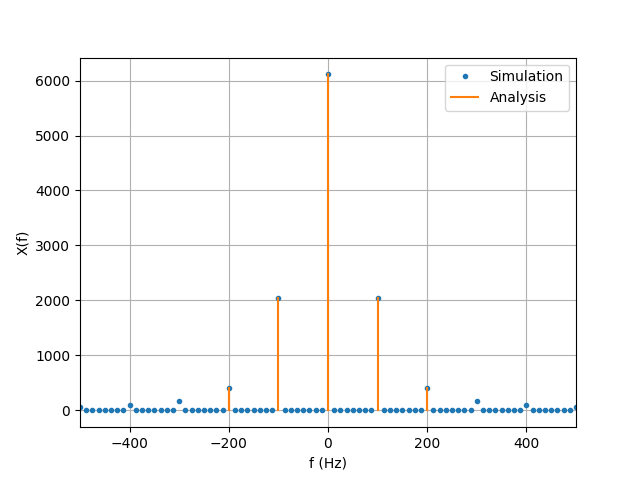
\includegraphics[width=\columnwidth]{figs/3_8.png}
    \caption{Fourier Transform of $x(t)$.}
    \label{eq:fig-fourier-xt}
\end{figure}
\item Show that
\begin{align}
    \rect{t} \system{F} \sinc{t}
\end{align}
Verify using python.

\solution We write
\begin{align}
    \rect{t}&\system{F}\int_{-\infty}^{\infty}\rect{t}e^{-\j2\pi ft}\, dt \\
            &=\int_{-\frac{1}{2}}^{\frac{1}{2}}e^{-\j2\pi ft}\, dt \\
            &=\frac{e^{\j\pi f} - e^{-\j\pi f}}{\j2\pi f} = \frac{\sin{\pi f}}{\pi f} = \sinc{f}
            \label{eq:fourier-rect}
\end{align}
The python code \texttt{codes/3\_9.py} verifies \eqref{eq:fourier-rect}.
\begin{figure}[!ht]
    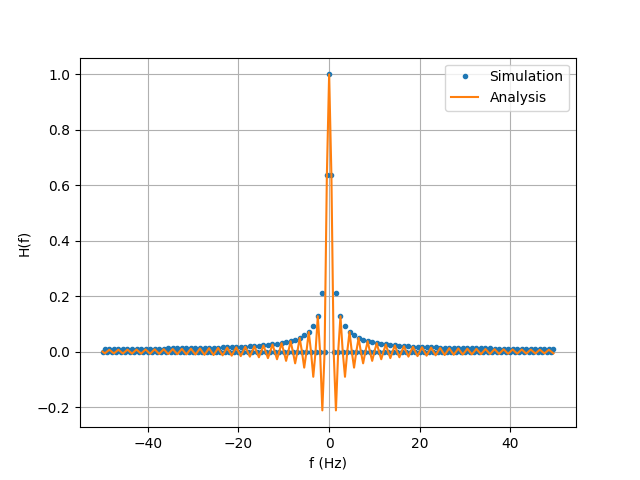
\includegraphics[width=\columnwidth]{figs/3_9.png}
    \caption{Fourier Transform of $\rect(t)$.}
    \label{eq:fig-fourier-rect}
\end{figure}
\item $\sinc{t}\system{F} ?$  Verify using python.

\solution From \eqref{eq:duality}, we have 
\begin{align}
    \sinc{t}\system{F}\rect(-f)=\rect{f}
    \label{eq:fourier-sinc}
\end{align}
Since $\rect{f}$ is an even function.
The python code \texttt{codes/3\_10.py} verifies \eqref{eq:fourier-sinc}.
\begin{figure}[!ht]
    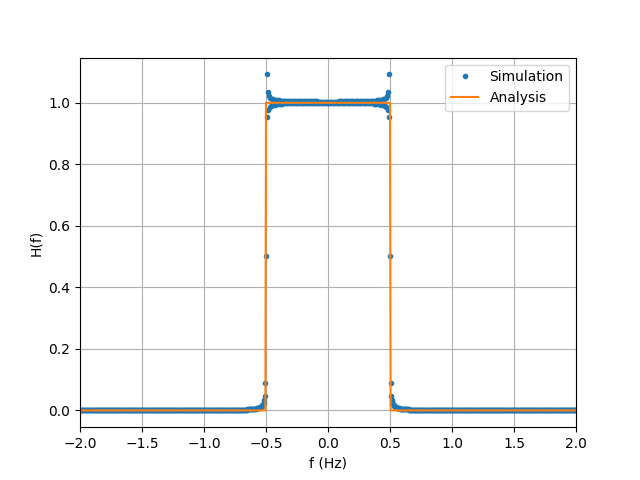
\includegraphics[width=\columnwidth]{figs/3_10.png}
    \caption{Fourier Transform of $\sinc(t)$.}
    \label{eq:fig-fourier-sinc}
\end{figure}
\end{enumerate}

\section{Filter}
\begin{enumerate}[label=\thesection.\arabic*
,ref=\thesection.\theenumi]
\item Find $H(f)$ which transforms $x(t)$ to DC 5V.
The function $H(f)$ is a low pass filter which filters around the
zero frequency component. The rectangular function represents an ideal
low pass filter. Note that
\begin{align}
    \rect{\frac{f}{4f_0}} = 
    \begin{cases}
        1 & \abs{f} < 2f_0 \\
        0 & \textrm{otherwise}
    \end{cases}
\end{align}
and hence from \eqref{eq:fourier-xt},
\begin{align}
    H(f) = \frac{\pi V_0}{2A_0}\rect\brak{\frac{f}{4f_0}}
    \label{eq:Hf}
\end{align}
where $V_0 =$ 5V.

\item Find $h(t)$.

\solution Suppose $g(t)\system{F}G(f)$. Then, for some
nonzero $a \in \mathbb{R}$
\begin{align}
    g(at)&\system{F}\int_{-\infty}^{\infty}g(at)e^{-\j2\pi ft}\, dt \\
         &=\frac{1}{a}\int_{-\infty}^{\infty}g(u)e^{\brak{-\j2\pi \frac{f}{a}t}}\, dt \\
         &=\frac{1}{a}G\brak{\frac{f}{a}}
         \label{eq:t-scaling}
\end{align}
where we have substituted $u := at$. Using 
\eqref{eq:t-scaling} of the Fourier Transform in \eqref{eq:Hf},
\begin{align}
    h(t) = \frac{2\pi f_0V_0}{A_0}\sinc\brak{4f_0t}
\end{align}
\item Verify your result using convolution.

\solution The Python code \texttt{codes/4\_3.py} verifies the result
by plotting the graph below.
\begin{figure}[!ht]
    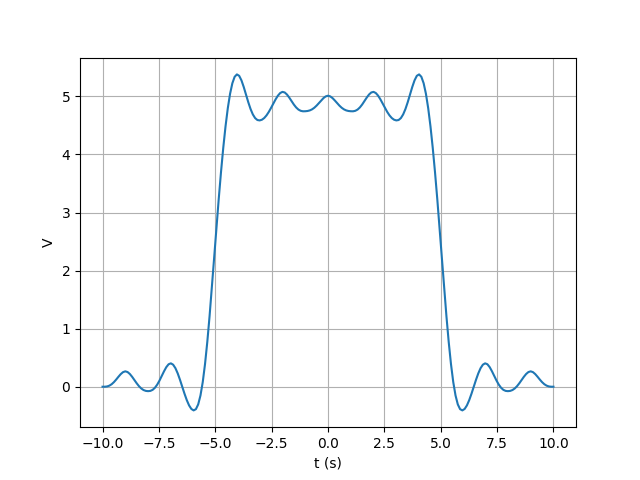
\includegraphics[width=\columnwidth]{figs/4_3.png}
    \caption{Convolution of the two signals.}
    \label{eq:fig-conv}
\end{figure}
\end{enumerate}
\section{Filter Design}
\begin{enumerate}[label=\thesection.\arabic*
,ref=\thesection.\theenumi]
\item Design a Butterworth filter for $H(f)$.

\solution
\item Design a Chebyschev filter for $H(f)$.

\solution
\item Design a circuit for your Butterworth filter.

\solution
\item Design a circuit for your Chebyschev filter.

\solution
\end{enumerate}
\end{document}
